Algunas aplicaciones de la distancia euclidiana incluyen:

\begin{enumerate}
\item \textbf{ Algoritmos de búsqueda y optimización:} La distancia euclidiana se utiliza en algoritmos de búsqueda para encontrar la ruta más corta entre dos puntos en un espacio euclidiano. También se utiliza en algoritmos de optimización para minimizar la distancia entre puntos en un espacio multidimensional.
\item \textbf{ Análisis de redes de transporte:} En el análisis de redes de transporte, la distancia euclidiana se utiliza para calcular la distancia entre nodos o puntos de interés en una red de carreteras, ferrocarriles, o rutas de transporte público.
\item \textbf{Problemas de asignación de recursos:} En problemas de asignación de recursos, la distancia euclidiana se utiliza para calcular la distancia entre diferentes ubicaciones o recursos, lo que puede ayudar a optimizar la asignación de recursos en un espacio geográfico.
\end{enumerate}

En resumen, la distancia euclidiana es una medida comúnmente utilizada en aplicaciones donde se requiere calcular distancias en un espacio euclidiano y donde los movimientos no están restringidos a movimientos verticales y horizontales, como en el caso de la distancia de Manhattan.

En el contexto de aplicaciones, la distancia de Manhattan se utiliza en diversas áreas, como en algoritmos de búsqueda y optimización, en análisis de redes de transporte y en problemas de asignación de recursos. Por ejemplo, en logística, la distancia de Manhattan puede utilizarse para calcular la distancia entre dos ubicaciones en una ciudad, considerando solo los movimientos horizontales y verticales.

En resumen, la distancia de Manhattan es una medida útil en aplicaciones donde se necesita calcular distancias en un espacio cartesiano y donde los movimientos están restringidos a movimientos verticales y horizontales.

Algunas aplicaciones de la distancia esférica incluyen:

\begin{enumerate}
	\item \textbf{Sistemas de navegación:} La distancia esférica se utiliza en sistemas de navegación para calcular la distancia entre dos puntos en la superficie de la Tierra, lo que ayuda a determinar la ruta más corta entre dos ubicaciones.
	\item \textbf{Geolocalización:} En aplicaciones de geolocalización, la distancia esférica se utiliza para calcular la distancia entre la ubicación actual de un dispositivo y puntos de interés cercanos, como restaurantes, tiendas, o eventos.
	\item \text{Astronomía:} En astronomía, la distancia esférica se utiliza para medir la distancia entre objetos celestes, como estrellas, planetas, o galaxias, que están ubicados en el espacio tridimensional.
\end{enumerate}

En resumen, la distancia esférica es una medida comúnmente utilizada en aplicaciones donde se requiere calcular distancias en la superficie de la Tierra o en el espacio tridimensional, como en el caso de la navegación, geolocalización y astronomía.

\subsection{Coordenadas giratorias}

Algunos problemas son más fáciles de resolver si se usan distancias de Manhattan en lugar de distancias euclidianas. Como ejemplo, considere un problema en el que se nos da n puntos en el plano bidimensional y nuestra tarea es calcular la distancia máxima de Manhattan entre dos puntos. Por ejemplo, considere el siguiente conjunto de puntos:

% TODO: \usepackage{graphicx} required
\begin{figure}[!h]
	\centering
	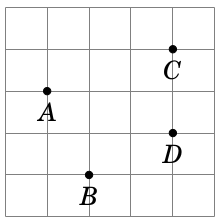
\includegraphics[width=0.25\linewidth]{img/diistance_functios_1}
	\label{fig:diistancefunctios1}
\end{figure}

La distancia máxima de Manhattan es 5 entre los puntos $B$ y $C$:

\begin{figure}[!h]
	\centering
	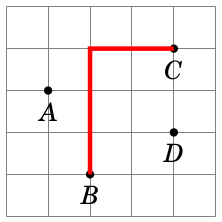
\includegraphics[width=0.25\linewidth]{img/diistance_functios_2}
	\label{fig:diistancefunctios2}
\end{figure}

Una técnica útil relacionada con las distancias de Manhattan es rotar todas las coordenadas 45 grados para que se convierta un punto $(x,y)$ a $(x + y, y - x)$. Por ejemplo, después de rotar los puntos anteriores, el resultado es:

\begin{figure}[!h]
	\centering
	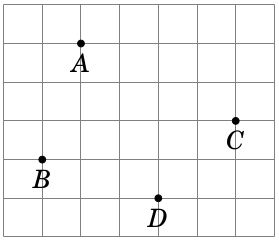
\includegraphics[width=0.25\linewidth]{img/diistance_functios_3}
	\label{fig:diistancefunctios3}
\end{figure}

Y la distancia máxima es la siguiente:

\begin{figure}[!h]
	\centering
	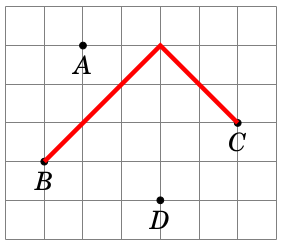
\includegraphics[width=0.25\linewidth]{img/diistance_functios_4}
	\label{fig:diistancefunctios4}
\end{figure}

Considere dos puntos $P_1 = (x_1, y_1)$ y $P_2 = (x_2, y_2)$ cuyas coordenadas rotadas son $P'_1 = (x'_1, y'_1)$ y $P'_2 = (x'_2, y'_2)$. Ahora hay dos formas de expresar la distancia de Manhattan entre $P_1$ y $P_2$:

$$|x_1-x_2|+|y_1-y_2| = \max (|x'_1-x'_2|,|y'_1-y'_2|)$$

Por ejemplo, si $P_1=(1,0)$ y $P_2=(3,3)$, las coordenadas rotadas son $P'_1=(1,-1)$ y $P'_=(6,0)$ y la distancia de Manhattan es

$$|1-3| + |0-3| = \max(|1-6|, |-1-0|) = 5$$

Las coordenadas rotadas proporcionan una forma simple de operar con distancias de Manhattan, porque podemos considerar las coordenadas X e Y por separado. Para maximizar la distancia de Manhattan entre dos puntos, debemos encontrar dos puntos cuyas coordenadas rotadas maximizan el valor de:

$$ \max (|x'_1-x'_2|,|y'_1-y'_2|) $$

Esto es fácil, porque la diferencia horizontal o vertical de las coordenadas rotadas tiene que ser máxima.

